\documentclass[conference]{IEEEtran}[10pt]


\makeatletter
\def\ps@headings{%
\def\@oddhead{\mbox{}\scriptsize\rightmark \hfil \thepage}%
\def\@evenhead{\scriptsize\thepage \hfil \leftmark\mbox{}}%
\def\@oddfoot{}%
\def\@evenfoot{}}
\makeatother \pagestyle{headings}

\makeatletter
\def\ps@headings{%
\def\@oddhead{\mbox{}\scriptsize\rightmark \hfil \thepage}%
\def\@evenhead{\scriptsize\thepage \hfil \leftmark\mbox{}}%
\def\@oddfoot{}%
\def\@evenfoot{}}
\makeatother \pagestyle{headings}


\usepackage{cite}
\usepackage{times}
%\usepackage{dsfont}

\usepackage{graphicx}
\usepackage{epstopdf}
\usepackage{subfigure}
\usepackage{color}
\usepackage{ifpdf}
%\usepackage{subfig}
\usepackage{epsfig}
\usepackage{latexsym}
\usepackage{amsfonts}
\usepackage{amssymb}
\usepackage{paralist}
\usepackage{comment}
\usepackage{xspace}
\usepackage{mathrsfs}
\usepackage{amssymb}
\usepackage{slashbox}
\usepackage{setspace}
\usepackage{color}
\usepackage[small]{caption2}

\usepackage{algorithm}
%\usepackage{algorithmic}
%\usepackage[linesnumbered,boxed]{algorithm2e}
%\usepackage[ruled]{algorithm}
\usepackage[noend]{algorithmic}
\usepackage{algorithmic}

\usepackage{amssymb}
\usepackage{url,epsfig,array}
\usepackage{leftidx}
\usepackage{amsmath}

\usepackage[
top=0.85in, bottom=0.85in,
left=0.75in, right=0.75in
  %pass,% keep layout unchanged
  % showframe,% show the layout
]{geometry}

% correct bad hyphenation here
\hyphenation{optical networks semi-conductor}

\def\ie{\textit{i.e.}\xspace}
\def\etal{\textit{et al.}\xspace}
\def\etc{\textit{etc.}\xspace}
\def\whp{\textit{w.h.p.}\xspace}
\def\eg{\textit{e.g.}\xspace}
\def\iid{\textit{i.i.d.}\xspace}
\def\st{\xspace\textbf{s.t.}\xspace}

\newtheorem{theorem}{Theorem}
\newtheorem{axiom}[theorem]{Axiom}
\newtheorem{corollary}[theorem]{Corollary}
\newtheorem{definition}{Definition}
\newtheorem{lemma}[theorem]{Lemma}
%\newtheorem{theorem}[theorem]{Theorem}
\newtheorem{remark}[theorem]{Remark}
\newtheorem{protocol}{Protocol}

\def\sharedaffiliation{%
\end{tabular}
\begin{tabular}{c}}

\newcommand{\tabincell}[2]{\begin{tabular}{@{}#1@{}}#2\end{tabular}}

\newcommand{\hint}{\texttt{hint()}}

\setlength{\abovedisplayskip}{1pt}
\setlength{\belowdisplayskip}{1pt}

\renewcommand{\algorithmicrequire}{\textbf{Input:}}
\renewcommand{\algorithmicensure}{\textbf{Output:}}
\newcommand{\argmax}{\operatornamewithlimits{argmax}}

\newcommand{\linote}[1]{{$\langle${\textcolor{red}{\textbf{#1}}}$\rangle$}}
\newcommand{\mynote}[1]{{$\langle${\textcolor{blue}{\textbf{#1}}}$\rangle$}}

\begin{document}

%
% paper title
% can use linebreaks \\ within to get better formatting as desired
\title{Integrating Coflow and Circuits Scheduling for Optical Networks}
%\title{Joint Optimization of Control Plane and Data Plane in SDNs with Multiple Controllers}

% author names and affiliations
% use a multiple column layout for up to three different
% affiliations
%\author{\IEEEauthorblockN{Conference Subsmission$^1$} }

\author{\IEEEauthorblockN{IEEE INFOCOM 2018, Paper \# } }

\maketitle
%\author{\IEEEauthorblockN{IEEE IWQoS 2017 Submission, Paper \# 1570347180} }
\begin{abstract}
%\boldmath
Optical Circuit Switches (OCS) are increasingly used in cluster networks due to their data rate, energy and longevity advantages over electrical packet switches. Concurrently, an emerging crucial requirement for modern data-parallel clusters is to achieve high application-level communication efficiency when servicing structured traffic flows (a.k.a. Coflows) from distributed data processing applications. Only completing all flows in a coflow is meaningful to an application. To optimize application performance, both traffic scheduling and switch scheduling must be jointly considered at the level of a coflow rather than individual flows. However, prior solutions have significant limitation: they only consider traffic scheduling in the traditional network, or consider the switch scheduling for only one switch, which are both insufficient. To this end, we present TSS, a coflow-aware network optimization framework that seamlessly integrates traffic and switch scheduling for better application performance. Using a large-scale simulations, we demonstrate that TSS significantly reduces the average coflow completion time (CCT) by up to 66.3\% compared to the state-of-the-art scheduling-only solution.

\end{abstract}

\begin{IEEEkeywords}
\emph{Coflow, Routing and scheduling, OCS.}
\end{IEEEkeywords}
\begin{comment}

\author{\IEEEauthorblockN{Hongli Xu$^1$ \   Liusheng Huang$^1$}
\IEEEauthorblockA{Email:
xuhongli@ustc.edu.cn, lshuang@ustc.edu.cn\\
$^1$ School of Computer Science and Technology, University of
Science and Technology of China, China } }
%\IEEEauthorblockN{Liusheng Huang\\
%and Montgomery Scott}
%\IEEEauthorblockA{Starfleet Academy\\
%San Francisco, California 96678-2391\\
%Telephone: (800) 555--1212\\
%Fax: (888) 555--1212}}
\end{comment}
% make the title area


\section{Introduction}\label{sec:intro}
Optical circuit switches (OCS) are increasingly used in cluster networks because of the robustness, high link bandwidth and low energy consumption. In an optical circuit switch network, a connection is set up by establishing a lightpath from the source node to the destination node. A lightpath is an optical channel that may span multiple fiber links to provide a circuit-switched interconnection between two nodes which avoids the expensive optical-electrical-optical conversions and makes the high bandwidth available. Apart from these advantages, an OCS has two constraints. First, and input (output) port can set up at most one circuit to an output (input) port at a time. That is, no input (output) port may connect to multiple output (input) ports. Second, each circuit can be reconfigured with a fixed time delay $\delta$, which means it takes time $\delta$ to set up a new circuit and during the period of $\delta$, the communication stops on the the input (output) ports on the circuits to be set up or torn down. However, other circuits remain unchanged and keep working.


Cluster computing frameworks such as MapReduce \cite{dean2008mapreduce}, Dryad \cite{isard2007dryad}, Spark \cite{zaharia2010spark} and so on have become the mainstream platforms for data processing and analysis in today’s cloud services. A common feature of these different computing paradigms is that they all implement a data flow computing model, in which a group of data flows need to pass through a sequence of intermediate processing stages before generating the final results. These intermediate flow transfers can account for more than 50\% of job completion time \cite{chowdhury2011managing}, and have a significant impact on job performance. Therefore, optimizing such flow transfers is important for applications. The term coflow is defined as the set of all flows transferring data between two stages of a job \cite{zhao2015rapier}. To optimize application performance, we need to optimize flow transfers at the level of coflow rather than individual ones. This is because the job completion time depends on the time it takes to complete the entire coflow, instead of the time to complete individual flows composing it. For example, in MapReduce \cite{dean2008mapreduce} and BSP \cite{cheatham1996bulk}, a stage cannot complete, or sometimes even start, before it receives all the flows in a coflow from the previous stage. From an application’s perspective, when a stage is pending for the input data, the CPU often sits idle or is under-utilized. As a result, reducing the coflow completion time (CCT) can further improve CPU utilization, maximizing application performance and job throughput in a given time period.



Recently, some studies \cite{chowdhury2012coflow} \cite{chowdhury2014efficient} \cite{dogar2014decentralized} have devoted on minimizing average CCT. These works can be mainly divided into two main categories. However, we demonstrate that both two categories be insufficient for scheduling optimization, especially for multi-hop OCS, which will reduce the user's QoS. One category is the Coflow scheduling through routing and scheduling in the traditional network \cite{zhao2015rapier}. First, since this work only focuses on the traditional (or non-optical) network, this method does not consider the switch scheduling for coflow scheduling. Second, due to the optical switching feature, the route path between two devices in the optical network is time aware. As a result, the result for the traditional network can not work well for the optical network. The second categories is called Sunflow \cite{huang2016sunflow}, which studies the switch scheduling on one switch for minimizing CCT. First, this work does not consider the impact of flow routing and traffic scheduling on the CCT. Second, this work only considers the case with one switch, thus it is difficult to be extended to the general multi-hop optical network.



Therefore, \textit{it is an urgent need to minimize CCT by joint optimization of traffic scheduling and switch scheduling in the optical networks}. The main contributions of this paper are:
\begin{enumerate}
\item We formulate the problem of how to determine which feasible lightpaths and when to forward
flows and schedule the OCS network to minimize the coflow completion time (CCT). The NP-hardness is also analyzed.
\item To solve this problem, we separate this problem into two subproblems and prove their NP-hardness. For the first subproblem, we given an approximation algorithm with approximation ratio $\frac{4}{3}-\frac{1}{3k}$, where $k$ is the number of feasible lightpaths per ToR switch pair. For the second subproblem,  we given an approximation algorithm with approximation ratio $h$, where $h$ is  h is the maximum hop count of all the lightpaths.
%\item We propose the maximum flow statistics collection (MFSC) with cost constraint problem, and prove its NP-hardness. To clarify this problem, we also discuss the difference from the previous problems, and show that there is no polynomial-time algorithm with approximation ratio $1- e^{-1} + \epsilon $ unless $NP \subseteq DTIME(n^{\log\log n})$, where $\epsilon $ is an arbitrarily small value.

\item We evaluate the proposed algorithms with simulations. The simulation results show that our algorithms can reduce the CCT about 40-80\% compared with the Baseline. %Moreover, our partial FSC algorithm reduces the cost by 52\% compared with FSC while preserving almost the similar application performance.
\end{enumerate}



The rest of this paper is organized as follows. Section \ref{sec:prelim} formalizes the COCIS problem, and gives the NP-hardness proof. In Section \ref{sec:design}, we separate COCIS into two subproblems and propose corresponding approximation algorithms. The approximation ratios are also analyzed in this section. The simulation results are reported in Section \ref{sec:evaluation}. In Section \ref{sec:relwork}, we introduce the related works. We conclude the paper in Section \ref{sec:conclusion}.



\section{Problem Formulation}\label{sec:prelim}
\subsection{Network Model}\label{sec:networkmodel}
We start with the conceptional model used to study the scheduling algorithm. In an optical circuit switched (OCS) network, the switch ports are connected to Top-of-Rack (ToR) switches, and each ToR switch is connected to $k$ machines. The link bandwidth is $B$. The source and destination nodes of a flow are ToR switches. Each ToR switch can serve as a source and destination simultaneously. We assume no buffering in the optical circuit switched netowrk, hence all the buffering occurs in the edge of the network, i.e. with the ToR switches. A flow can be forwarded only when the lightpath is set up between the source node and the destination node. In this article, the optical circuit switched (OCS) network and optical network are the same meaning.

With this network model, we have the following assumptions for the network.

\begin{itemize}
\item Each source-destination ToR switch pair has $k$ feasible lightpaths. Since a ToR switch has $k$ output ports which are connected to $k$ machines, we assume that the $k$ feasible lightpaths exist. What's more, if $k$ feasible lightpaths are in the same port of a ToR, these lightpaths will be no big difference with a single lightpath and these lightpaths even need a extra delay during circuits reconfiguration. On this account, we assume that the these $k$ lightpaths will pass through different ports of the ToR switch pair. For a ToR switch pair $(i.j)$, the $k$-feasible lightpath set is denoted as $P_{i,j}$. The feasible lightpath set for all ToR switch pairs is denoted by $P=\bigcup_{i,j}P_{i,j}$.  
\item Inspired by \cite{chowdhury2011managing} \cite{chowdhury2014efficient}, we assume that our network runs in a centralized manner, which accords with many recent centralized optical networks \cite{simeonidou2013software} \cite{ramamurthy2002fixed}. In this paper, we assume that the information about a coflow is given and the central scheduler can control all the switches in the network. 
\end{itemize}

\subsection{Traffic Model}\label:{sec:trafficmodel}
In this part, we focus on the traffic model called $\emph{coflow}$, which is defined as the set of all flows transferring between two stages of a job. Because the ToR switch is not just a host, there may be more than one flows from ToR switch $i$ to ToR switch $j$. A flow set of a coflow can be denoted as $C$, where each element $\Gamma_{i,j}\in C$ indicates flow set $\Gamma_{i,j}$ that include all flows from ToR switch $i$ to ToR switch $j$. Note that $|C|$ is the number of flows in a coflow $C$. Denote $f_{i,j}^m$ as the $m^{th}$ flow of $\Gamma_{i,j}$ and $d_{i,j}^m$ as the amount of data of $f_{i,j}^m$. In this paper the flow is unsplittable. %If not mentioned, the flow is interruptible \cite{huang2016sunflow}.

Combined with the Section \ref{sec:networkmodel}, we have some remarks. In the network model, there is a feasible ligthpath set $P_{i,j}$ for a source-destination ToR switch pair $(i,j)$. Likewise, there is a flow set $\Gamma_{i,j}=\{f_{i,j}^1,f_{i,j}^2,...,f_{i,j}^m\}$ for the ToR switch pair $(i,j)$. That is, for each flow set $f_{i,j}$, there corresponds a lightpath set $P_{i,j}$.
\subsection{Routing and Scheduling Objective}\label{sec:objective}
For a coflow $C$, the objective is to minimize the Coflow Completion Time (CCT), which is the duration to finish all the flows in a coflow, so as to speed up application level performance. To achieve this goal, we propose two notions as follows.
\begin{itemize}



\item \textbf{Feasible lightpath set:} For a flow set $\Gamma_{i,j}$, there may be more than one lightpath from ToR switch $i$ to $j$. combined with the assumption in \ref{sec:networkmodel}, the feasible lightpath set has $k$ feasible paths. Denote $P_{i,j}$ as the feasible path set of flow set $\Gamma_{i,j}$.
\item \textbf{Active period for a lightpath:} Because of the OCS network scheme, a lightpaths in our network model changes when a new circuit is set up or the former circuit is torn down. So a lightpath lasts for a period, called ``active period". It's worth noting that an active period is an interval and the interval length is the \textbf{duration} for a lightpath.
\end{itemize}

With these notions, we illustrate our problem. Our objective is to minimize the coflow completion time (CCT). What we know are network model and coflow information. We need to determine which feasible lightpaths and when to forward flows. Besides, we need to schedule the OCS network to finish the transmission of a coflow. So our problem is called \textbf{Coflow and Circuits Scheduling problem (COCIS)}.

The COCIS problem is NP-hard. Furthermore, we will show the two subproblems, coflow scheduling (COS) and circuits scheduling (CIS), are NP-hard too. The COS problem is a special case that the circuits scheduling in the OCS network is fixed. Likewise, the CIS problem is the special case that the coflow routing and scheduling are fixed. After we prove that COS and CIS are NP-hard, COCIS is NP-hard too.


%\subsubsection{Interruptible Coflow Routing and Scheduling(ICRS)}
\begin{comment}An interruptible flow spans multiple active period. That is, for an interruptible flow, an active period in a lightpath with unfinished transmission demand incurs extra active periods to continue the transmission. Interruptible flows are widely applied in classical networks, especially the networks with reliable communications protocols such as TCP.

In an OCS network, the interruptible flows are still very common \cite{huang2016sunflow}. In order to minimize the CCT, for each flow $f_{i,j}^k\in f_{i,j}$ and each $f_{i,j}\in C$, we need to choose a period $[t_p^{start},t_p^{end}]\in T_{i,j}$ and determine the start time $t_{f_{i,j}^k}^{start}$ for $f_{i,j}$ that satisfies:
\begin{equation}\label{formu_1}
\begin{aligned}
t_{f_{i,j}^k}^{start}&\geq t_{f_{i,j}^k}^{permitted}\\
 t_p^{start} \leq &t_{f_{i,j}^k}^{start}\leq t_p^{end}\\
 \end{aligned}
 \end{equation}

Note that $t_{f_{i,j}^k}^{permitted}$ is the permitted start time for ${f_{i,j}^k}$. For example, when part of a flow is transmitted, the remaining part can only be allowed to transmitted after that. The second inequalities in Eq. \ref{formu_1} mean that the flows should be forwarded in the active period. Once a flow transmission is finished, the active time need to de updated. Likewise, once the transmission is not finished and the the active period is over, the amount of data of the flow should be updated. Our objective is:
 \begin{equation}\label{objective_1}
 \begin{aligned}
 \min \ \ & t  \\
 t_{f_{i,j}^k}^{start}+\frac{d_{i,j}^k}{B}&\leq t, \qquad\forall f_{i,j}^k\\
 \end{aligned}
 \end{equation}
\end{comment}
%\subsubsection{Non-Interruptible Coflow Routing and Scheduling(NICRS)}
\begin{comment}
An non-interruptible flow, should be forwarded within a single active period. In an OCS network with UDP, the sender has no idea about the change of lightpath and continues it's transmission, which is useless and results in the transmission failure. To avoid this type of failure, the assumption that the flow is non-interruptible is necessary.



In order to minimize the CCT, for each flow $f_{i,j}^k\in f_{i,j},f_{i,j}\in C$, we need to choose a period $[t_p^{start},t_p^{end}]\in T_{i,j}$ and determine the start time $t_{f_{i,j}^k}^{start}$ for $f_{i,j}$ that satisfies:
\begin{equation}\label{formu_2}
\begin{aligned}
 t_{f_{i,j}^k}^{start}+\frac{d_{i,j}^k}{B}&\leq t_p^{end}\\
 t_{f_{i,j}^k}^{start}&\geq t_p^{start}\\
 \end{aligned}
 \end{equation}

The above inequalities mean that the flows should be forwarded and the transmission is finished in the active period. Once a flow transmission is finished, the active period needs to be updated. Our objective is:
 \begin{equation}\label{objective_2}
 \begin{aligned}
 \min \ \ & t  \\
 t_{f_{i,j}^k}^{start}+\frac{d_{i,j}^k}{B}&\leq t, \qquad\forall f_{i,j}^k\\
 \end{aligned}
 \end{equation}
\end{comment}

\begin{theorem}\label{COS:nphard}
The COS problem is NP-hard.
\end{theorem}

\begin{theorem}\label{CIS:nphard}
The CIS problem is NP-hard.
\end{theorem}

The proofs of lemmas \ref{COS:nphard} and \ref{CIS:nphard} have been relegated to the
Appendixes A and B, respectively.



\section{Algorithm and analysis}\label{sec:design}
In this section, we focus on the algorithm details for the COCIS problems. COCIS is a joint optimization of coflow and OCS network to minimize the CCT. As we can see in \ref{sec:objective}, not only COCIS but also two subproblems of COCIS are NP-hard. In view of the complexity and difficulty of the COCIS problem, we separate our framework into two steps, which will be introduced in \ref{sec:framework}.

The rest of the algorithm section is organized as follows. Section \ref{sec:framework} shows the overall framework of our algorithm. In section \ref{sec:alg_coflow}, we introduce the first step our framework, which aims at coflow routing and scheduling. Section \ref{sec:alg_circuit} introduces the second step of our framework. Finally, section \ref{discussion} discusses some other things about our algorithms.
\subsection{Framework}\label{sec:framework}
In this part, we give the overall description of our framework. We separate our framework into two steps. First, we determine the route from the $k$ feasible lightpath set and the order distribution of each flow in the same lightpath. Second, given the route and duration of each lightpath, we schedule the circuits in the OCS network. Our framework is shown in Alg. \ref{alg:framework}.
{\small
\begin{algorithm}
\caption{ Framework     }\label{alg:framework}
\begin{algorithmic}[1]
%\STATE {\textbf{Input: }
\STATE {\textbf{Step 1:Coflow Routing and Order Distribution} /*  determine a lightpath for each flow in coflow $C$ and the order for flows in the same lightpath */ }

\STATE {\textbf{Step 2: Circuits Scheduling for Each Lightpath} /* assign each lightpath an active time whose length is the duration in step 1 */ }

\end{algorithmic}
\end{algorithm}
}


The first step is coflow routing and order distribution. It aims at scheduling the coflow. Each flow has $k$-feasible lightpaths and coflow routing will determine which lightpath the flow will pass through. That is, our coflow scheduling includes routing and order distribution. If multiple flows pass through the same lightpath, the forwarding order is another problem. It's what the order distribution does. After appointing all the flows in $C$, we will compute the duration of each lightpath, which is the input of step 2. The second step in the framework get the duration of each lightpath. It will schedule the circuits of the whole network to minimize the CCT and output the scheduling scheme. Each lightpath will have an active period whose interval length is its duration. Because step 2 appoints each lightpath the exact duration. So the order in the same lightpath can be changed. That is, we only need to know the duration of each ligthpath. However, in the practical implementation of step 1, we do have an order for each flow to get a better approximation performance.
%\subsection{Approximation Bound Analysis for IRSC}


%\subsection{Non-Interruptible Routing and Scheduling for Coflows (NIRSC)}
\subsection{Greedy Routing and Order Distribution (GROD)\& Analysis }\label{sec:alg_coflow}
We introduce step 1 of our framework. Given the Coflow $C$ and the feasible lightpath set for a source-destination ToR pair, we assign each ligthpath a number of flows with an greedy algorithm. There might be an exponential number of feasible lightpaths between a source ToR switch and a destination ToR switch. Following \cite{hong2013achieving} \cite{al2010hedera}, we assume that the central scheduler has pre-computed $k$ feasible lightpaths between each pair of ToR switches corresponding to the $k$ output port of a ToR switch. Note that $P=\bigcup_{i,j}P_{i,j}$ is the feasible lightpath set of the network. For a coflow, the algorithm will be executed iteratively until all the source-destination ToR pairs are traversed. It's worth noting that the routes of feasible lightpaths are ensured and the circuits scheduling that makes lightpaths active is the responsibility of step 2. There is a flow set for each ToR pair, for example, $\Gamma_{i,j}$. Without loss of generality, we use ToR pair $(i,j)$ and flow set $\Gamma_{i,j}$ as an example. For flow set $\Gamma_{i,j}=\{f_{i,j}^1,f_{i,j}^2,...f_{i,j}^m\}$ and feasible lightpath set $P_{i,j}=\{p_{i,j}^1,p_{i,j}^2,...,p_{i,j}^k\}$, the first step sorts all flows in $\Gamma_{i,j}$ non-increasingly according to their amount of data. In the second step, for each flow $f\in \Gamma_{i,j}$, appoint $f$ to the lightpath with the least duration. duration of a lightpath means the total processing time to forward the flows. Finally, the lightpath that is appointed a new flow will update the duration. The GROD algorithm outputs the required duration for each lightpath. The duration matrix is denoted by $T=\{t_{i,j,l}\}$.

{\small
\begin{algorithm}
\caption{GROD: Greedy Routing and Duration Assignment}\label{alg:GROD}
\begin{algorithmic}[2]
\STATE {\textbf{Input: $C$, $P_{i,j},\forall i,j$}}
\STATE {\textbf{Output: Duration Matrix $T$}}

%\STATE {\textbf{Step 1:Route and Duration Assignment (RDA) for Each Flow} /* for each flow in coflow $C$, determine a lightpath*/ }
\FOR {each $\Gamma_{i,j}\in C$}
    %\STATE {\textbf{Step 1:Route and Duration Assignment (RDA) for Each Flow}/* for each flow in coflow $C$, determine a lightpath*/ }
    \STATE {Initiate duration array $T_{i,j}\ =0$ for each element.}
    \STATE {Sort all flows in $\Gamma_{i,j}$ non-increasingly according to their amount of data}
    \FOR {each $f\in \Gamma_{i,j}$}
         \STATE {Assign the flow to the lightpath with the least duration in $P_{i,j}$}
         \STATE {Update the duration of the lightpath }
    \ENDFOR
\ENDFOR
%\STATE {\textbf{Step 1: For a fixed OCS network scheduling scheme, we construct an interruptible/non-interruptible routing and scheduling algorithm }}
%\STATE {\textbf{Step 2: Circuits Scheduling (CIS) for Each Lightpath} /*assign each lightpath an active time whose length is the duration in step 1*/ }

\end{algorithmic}
\end{algorithm}
}


\textbf{Approximation Bound Analysis for GROD.} We analyze the approximation performance of the proposed GROD algorithm. Because GROD is executed iteratively, the approximation bound will be the same for each source-destination ToR switch pair.  Without loss of generality, we use a source-destination ToR swtich pair $(i,j)$ as an example. Note that $GROD(I)$ is the maximum duration for $k$ lightpaths in $P_{i,j}$ with GROD and $OPT(I)$ is the optimal result when the input flow set is $I$. The approximation ratio is $R_{GROD}$.

\begin{theorem}\label{bound:GROD}
The approximation ratio $R_{GROD}\leq\frac{4}{3}-\frac{1}{3k}$.
\end{theorem}
\begin{IEEEproof}
If $k=1$, because $GROD(I)=OPT(I)$ and $\frac{4}{3}-\frac{1}{k}=1=\frac{GROD(I)}{OPT(I)}$.

For $k>1$, we assume that $I=\{f_1,f_2,...,f_m\}$ is the flow set with the least flow number that contradicts to the approximation ratio. The amount of data for the flows is $\{d_1,d_2,....d_m\}$, and the duration of flows are $\{t_1,...,t_m\}$. Thus the scheduling order is $\{f_1,f_2,...,f_m\}$ and the maximum duration of each lightpath is $GROD(I)$. We set the last finished flow is $f_{m_1}$ and $m_1=n$. Because if $m_1<n$, there exists another flow set $I'=\{f_1,f_2,...,f_{m_1}\}$ whose maximum duration is also $GROD(I)$. That is $GROD(I')=GROD(I)$.  However, it's optimal result $OPT(I')\leq OPT(I)$. So we have:
\begin{equation}
\frac{GROD(I')}{OPT(I')}\geq\frac{GROD(I)}{OPT(I)}> \frac{4}{3}-\frac{1}{3k}
\end{equation}

The above equation contradicts to our assumption that $I$ is the flow set with the least flow number that contradicts to the approximation ratio, so $m_1=m$. Now, we prove that if $I$ exists, $m\leq 2k$.

Because $f_m$ is the last finished flow, $f_m$ starts at $GROD(I)-t_m$. At that time, this lightpath had the least duration. So we have:
\begin{equation}
\begin{aligned}
GROD(I)-t_m  &\leq\frac{1}{k}\sum\limits_{q=1}^{m-1}t_q\\
GROD(I) &\leq\frac{1}{k}\sum\limits_{q=1}^{m}t_q+\frac{k-1}{k}t_m\\
\end{aligned}
\end{equation}

Combined with $OPT(I)\geq \sum\limits_{q=1}^{m}t_q$, we have:

\begin{equation}
\begin{aligned}
&\frac{4}{3}-\frac{1}{3k}\leq \frac{GROD(I)}{OPT(I)}\leq\frac{OPT(I)+\frac{k-1}{k}t_m}{OPT(I)}\\%=1+\frac{k-1}{k}\frac{t_m}{OPT(I)}\\
&\Rightarrow 4k-1<3k+3(k-1)\frac{t_m}{OPT(I)}\\
& \Rightarrow\ OPT(I)<3t_m
\end{aligned}
\end{equation}

Because $t_m$ is the least number among $\{t_1,...,t_m\}$, $m<2k$. Furthermore, we proof GROD is the optimal solution when $m<2k$. We set $m=2k$, since if $m\ne2k$, we set $t_q=0,\forall q=m+1,..,2k$. We set assume lightpath has two flows: $f_x$ and $f_y$. If $x,y\leq k$, there exists a lightpath whose two flows are $f_s,f_t,s,t>k$. Because $t_x,t_y\geq t_s,t_t$, we swap $t_y$ and $t_t$. Then $t_x+t_t\leq t_x+t_y$ and $t_s+t_y\leq t_x+t_y$. The scheduling scheme $O'$ after the swap is no big than the optimal solution, so $O'$ is an optimal solution too. For scheduling scheme $O'$, $f_1,...f_k$ are appointed to the $k$ different feasible lightpaths, so do $f_{k+1},...f_{2k}$. The scheduling scheme is the same as the GROD algorithm. So we have:
\begin{equation}
\frac{GROD(I)}{OPT(I)}=1\leq\frac{4}{3}-\frac{1}{3k}(k\geq2)
\end{equation}

In conclusion, on one hand, when $m=1$, GROD is the optimal solution, so the approximation ratio is $1$. On the other hand, when $m\geq2$, if there exists a counterexample $I$, $m$ must be no more than $2k$. Furthermore, we show GROD is the optimal solution if $m\leq2k$. We have proven that the counterexample $I$ doesn't exist, so lemma \ref{bound:GROD} is proved.
\end{IEEEproof}
\subsection{Circuits Scheduling \& Analysis}\label{sec:alg_circuit}
After the first step of the framework, we get the output: Duration matrix $T=\{t_{i,j,l}\}$. $t_{i,j,l}$ represents the duration of $l^{th}$ lightpath in $P_{i,j}$. In this section, we schedule the circuits in the OCS network to minimize the coflow completion time. Because the circuits scheduling will change the status of ports and lightpaths dynamically, we keep a table holding information about each lightpath and port of when they are free or busy, denoted by NST (Network Status Table). Once a port is released, we will search the lightpath set to find whether there exists a lightpath $p_{i,j,l}$ along which the ports are all free or not. If so, we will take up the ports and forward the flows until all the flows appointed to the lightpath are forwarded. What's more, lightpath $p_{i,j,l}$ will be excluded from the lightpath set and the NST will change the status of the lightpath $p_{i,j,l}$ and corresponding ports. Their status will be busy for the duration $t_{i,j,l}$. If not, we will wait until the next port is released. Our algorithm terminates when all the lightpath is excluded from lightpath set. Obviously, our loop can end because if there is lightpath remain in the lightpath set, it can at least wait until all the ports are free. Our circuits scheduling algorithm is given in Alg. \ref{alg:CIS}.
\begin{table}[!tp]
\begin{tabular}{c|c}
\hline
\hline
B& bandwidth of the link\\
\hline
$P\{p_{i,j,l}\}$&feasible lightpath set for all the ToR pairs\\
\hline
NST& Network Status Table\\
\hline
$Start(.)$& the start time of a lightpath\\
\hline
$End(.)$& the end time of a lightpath \\
\hline
$T=\{t_{i,j,l}\}$& duration matrix for the lightpath set $P$\\
\hline
$\delta$ &the reconfiguration time \\
\hline
$T_L$ &lower bound for the CCT\\
\hline
$T_O$ &CCT of optimal solution\\
\hline
$\Delta t_i$ &idle interval between $p_{i-1}$ and $p_i$\\
\hline
$h$ &the maximum hop count of lightpaths\\
\hline
\end{tabular}
\caption{Some Important Notations for Section \ref{sec:alg_circuit}}\label{tbl:notation}
\end{table}

\textbf{Approximation Bound Analysis for CIS.} Next, we analyze the circuits scheduling performance. In order not to conflict with the whole paper, \textbf{new notions in this section only suitable for this section}.

Before the analysis of approximation bound, we discuss the lower bound for our problem. For a port $j$, there are lightpath $p_1,p_2,...,p_N$ that pass through the port. Note that the transmission time is $t_1,...,t_1$. So the minimum time to finish the task is:
 \begin{equation}\label{eq:T_L}
 T_L^j=\sum\limits_{i=1}^{N}t_i
 \end{equation}

\begin{algorithm}
\caption{CIS: Circuits Scheduling Algorithm}\label{alg:CIS}
\begin{algorithmic}[3]
	\STATE $t$ = Begin time
	\WHILE{$P\ne \varnothing$}
	\FOR {$p_{i,j,l}$ in $P$}
	\STATE $temp=\delta+t_{i,j,l}$
	\STATE Search NST for all ports along the lightpath $P_{i,j,l}$
	\IF {all ports along $P_{i,j,l}$ is free at time $t$}
	\STATE Arrange lightpath $p_{i,j,l}$ to start at $t$ :
	\STATE $Start(p_{i,j,l})=t$
	\STATE $End(p_{i,j,l})=t+temp$
	\STATE Set lightpath $p_{i,j,l}$ is busy during $t$ to $t+temp$ in NST
	\FOR {each ports $p$ along the lightpath $p_{i,j,l}$}
	\STATE Set $p$ is busy during $t$ to $t+temp$ in NST
	\ENDFOR
	\STATE $P=P-p_{i,j,l}$
	\ENDIF
	\ENDFOR
	\STATE $t=$the next nearest release time in NST
	\ENDWHILE
\end{algorithmic}
\end{algorithm}



Note that the lower bound is $T_L$. we have:
\begin{equation}
T_L=\max\{T_L^1,T_L^2,...,\}
\end{equation}

\begin{theorem}\label{bound:CIS}
Algorithm CIS completes the transmission within $h$ times of the optimal solution, where $h$ is the maximum hop count of all the lightpaths.
\end{theorem}
\begin{IEEEproof}
Because a link connects to two ports, one input port and one output port, we use input port $j$ as an example. sort the lightpaths that pass through input port $j$ by the time they are scheduled to start transmission, denoted by $p_1,...,p_N$. $t_i$ denotes the time to transmit (including the reconfigure time delay $\delta$), and $\Delta t_i$ represents the idle interval between $p_{i-1}$ and $p_i$.

During $\Delta t_i$, port $j$ is idle. According to our algorithm, it means links of lightpath $f_i,f_{i+1},...,f_N$ are all busy during $\Delta t_i$ and at least one port of each lightpath is transmitting data for other lightpaths. Consider the last lightpath $p_N$, it has waited for $\sum\limits_{i=1}^{N}\Delta t_i$ totally. During the waiting time, the worst case is that all input ports, except port $j$, have finish their task. Combined with the lower bound, we know that a port finishes its task within $T_L$. Note that lightpath $p_N$ has $h_N$ input ports. We have:
\begin{equation}
\sum\limits_{i=1}^{N}\Delta t_i\leq (h_N-1)T_L\leq(h-1)T_L
\end{equation}


\begin{figure}
	\centering
    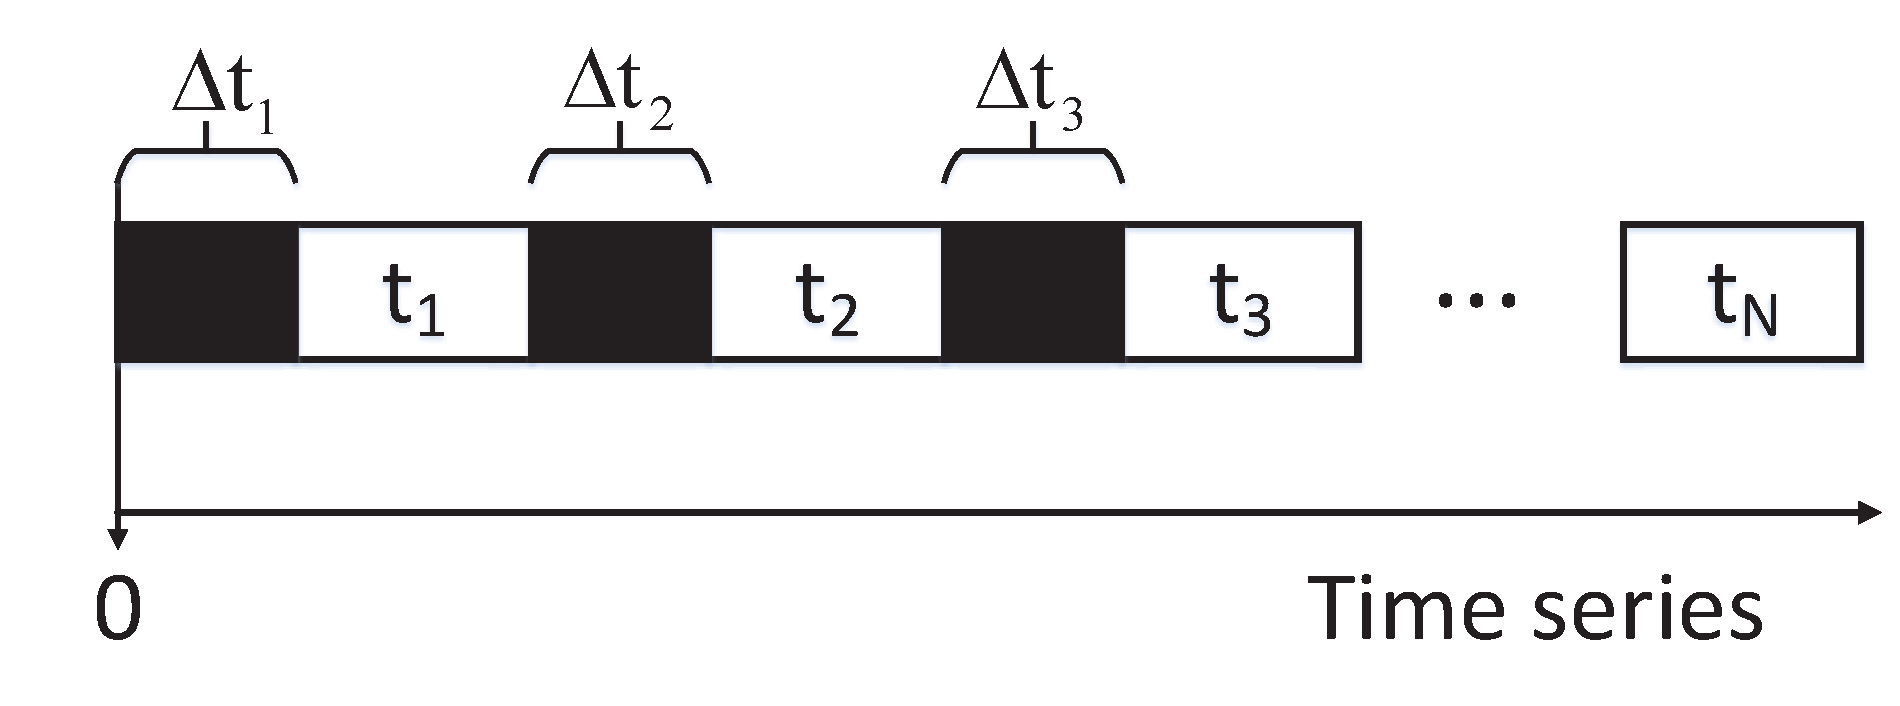
\includegraphics[width=0.45\textwidth]{timeline.eps}
	\caption{Timeline of a port}\label{fig:timeline}
\end{figure}

The transmission time of port $j$ is $\sum\limits{i=1}^N t_i$. According to Eq. \ref{eq:T_L}, we know:
\begin{equation}
\sum\limits_{i=1}^N t_i\leq T_L
 \end{equation}

So the completion time for port $j$ is:
\begin{equation}
\sum\limits_{i=1}^N t_i+\sum\limits_{i=1}^{N}\Delta t_i\leq (h-1)T_L+T_L=h T_L
\end{equation}

The completion time of the optimal solution is denoted by $T_O$. Because $T_L$ is lower bound to transmit the task, we have:
\begin{equation}
T_L<T_O
\end{equation}

The port $j$ is arbitrary, so algorithm CIS completes the transmission within $h$ times of the optimal solution. Lemma \ref{bound:CIS} is proved.

\end{IEEEproof}

\subsection{Time Conplexity}
In this section, we analyze the time complexity of GROD and CIS.

\begin{theorem}\label{time:GROD}
GROD's time complexity is $O(|\Gamma|\log m)$, where $m$ is the number of flows for each ToR switch pair.
\end{theorem}
\begin{IEEEproof}
GROD is executed for each ToR switch pair. For each pair $(i,j)$, there is a flow set $f_{i,j}$ and $|f_{i,j}|=m$. We sort the flow set with time complexity $O(m\log m)$, then appoint the flow with time complexity $O(m)$. So the total time complexity is $O(|\Gamma|(\log m+1))=O(|\Gamma|\log m )$.
\end{IEEEproof}
\begin{theorem}\label{time:CIS}
CIS's time complexity is $O(h|P|^2)$. Where $h$ is the maximum hop count of lightpaths.
\end{theorem}
\begin{IEEEproof}
The first loop is for all lightpaths in $P$. In the first loop, we first check the ports along the lightpath with time complexity $O(|P|h)$. After that we will go into the secong loop for all the lightpaths in $P$ with time complexity $O(|P|^2)$. In the second loop, we will check the ports along the lightpath with time complexity $O(h|P|^2)$. So the time complexity is $O(h|P|^2)$.
\end{IEEEproof}
\subsection{Discussion}\label{discussion}
The previous GROD and CIS algorithms are for intra-coflow scheduling. In this section, we will discuss inter-coflow scheduling. When multiple coflows compete for network resource, an important goal is to accommodate the network resource management policies for these coflows.

However, under different usage scenarios, we may need to use different management policies. For example, the policy may require that coflow requested by privileged users are preferred over that of regular users. Another example is that the policy may require the later-staged coflows yield to earlier-staged coflows to avoid the potential creation of stragglers that unnecessary prolong job runtime \cite{chowdhury2015efficient}. So the management is flexible and dependent on different constraints and objectives.

On the other hand, our GROD algorithm has already computed the required duration of each lightpath, and the CIS assign the lightpath the exact required duration. if we add a new task from another coflow, it may change the NST and furthermore increase the CCT of the original coflow. An stable way is to run each intra-coflow in order like \cite{huang2016sunflow}, which is one of the only a few researches that discussed the inter-coflow scheduling.
%\subsection{Approximation Bound Analysis for NIRSC}



\section{Evaluation}\label{sec:evaluation}
In this section, we will present the results from the large-scale simulation.
\subsection{Settings}
Our simulation adopt the two dimensional HyperX topology \cite{ahn2009hyperx}, which has 81 switches, each has attached to 16 other switches. Because our network is an optical network, the switches are optical circuit switches. There are multiple ToR switches each of which is connected to $k$ optical circuits switches. The link bandwidth $B=10Gbps$, which is the common link bandwidth in optical networks \cite{chatterjee2015routing} \cite{porter2013integrating}. The average flow size is $100Mbps$, which is almost equal to that of \cite{zhao2015rapier} in DCNs. In our simulation, we have two distribution for flows: 1)2-8 distribution, where twenty percent of flows are elephant flows and other eighty percent flows are mice flows. 2)Normal distribution, the average size of flows is $100Mbps$ \cite{antoniou2002log} \cite{dulman2003trade}. Our objective is to minimize the CCT. We will evaluate the impacts to CCT in four dimensions.

\begin{itemize}
\item \textbf{$k$, the number of feasible lightpaths for each ToR switch pair:} In our paper, we assume that each ToR switch is connected to $k$ optical circuit switches and each ToR switch pair has $k$ feasible lightpaths. In our simulation, we set $k=3,4,5,6$ and our default $k$ is 4.In the premise of not causing confusion, we omit the ``for each ToR witch pair" and say that \textbf{$k$ is the feasible lightpath number or the number of feasible lightpaths.}
\item \textbf{The number of ToR switches:} the ToR switches are access nodes of optical networks. If the ToR switches are sparse, the work load of the network will be light. If the ToR swtiches are dense, the work load of the lightpath will be heavy. In our simulation, we set the ToR switch number is 9-54. When the ToR switch number is 9 and feasible lightpath number $k$ is 3, only one in three optical circuit switches is connected to a ToR switch. When the ToR switch number is 54 and feasible lightpath number $k$ is 6, every optical switch is connected to 4 ToR switches. So our range of ToR switch number can cover different kinds of networks. Our default ToR switch number is 27.

\item \textbf{Reconfiguration delay $\delta$:} In optical networks, each circuit can be reconfigured with a fixed time delay $\delta$, In our simulation we set $\delta$=0.01ms,0.1ms,1ms,5ms and 10ms, where 10ms is the typical delay of  a 3D-MEMS optical switch \cite{huang2016sunflow} and 0.01ms is the delay of the latest research \cite{porter2013integrating}. In our simulation, we set the default time delay is 1ms, which is the accessible and common time delay for optical switches today.
\item \textbf{Flow number per ToR switch pair:} For each ToR switch pair, there is a flow set. In our simulation, we set the flow number per ToR switch pair is 10,20,30,40. Our default number is 20.
\end{itemize}


\subsection{Baseline for Comparison}

Because our paper focus on the coflow scheduling and circuits scheduling and our framework solves the problem in two steps: GROD and CIS. Here we introduce the baseline for GROD and CIS respectively.
\begin{itemize}
\item \textbf{Baseline for GROD}: GROD schedules each flow from the $k$ feasible lightpaths. A single way is to choose a fixed lightpath for each ToR switch pair. What's more, the less links the lightpath has, the less ports the lightpath will take up. So we choose the lightpath with the least hop count.
\item \textbf{Baseline for CIS}: CIS is to schedule the multiple optical circuit switches. As shown in Section \ref{sec:relwork}, most previous works focused on the scheduling of a single switch. We adopt the algorithm of Solstice \cite{liu2015scheduling} whose performance is significantly better than TMS and Edmond. To let Solstice be suitable for the multi-hop scheduling. We use the improved Solstice as the baseline for CIS.
\end{itemize}

After introducing the baseline for each step, we use four algorithms for comparison in our simulation. For ease of reading. The tabs and introductions of four algorithms are as follows. Because the tabs will be shown in the figures, so we will name the tabs as short as possible. For example, we wil use ``base" to represent the meaning of ``baseline".
\begin{itemize}
\item \textbf{GROD+CIS}: This is our proposed algorithm. We don't give unnecessary details.
\item \textbf{Base+CIS}: The first step is the baseline of GROD, and the second step is our CIS algorithm. We compare Base+CIS with GROD+CIS and Baseline.
\item \textbf{GROD+base}: The first step is CIS, and the second step is the baseline of GROD. We compare Base+CIS with GROD+CIS and Baseline
\item \textbf{Baseline}: Both of the two steps are baseline algorithms, so we call it the Baseline of GROD+CIS. if we name this algorithm like the above ones, it should be Base+Base. However, For ease of writing, we name it Baseline.
\end{itemize}



\begin{figure*}
\centering
\begin{minipage}[c]{0.23\textwidth}
\centering

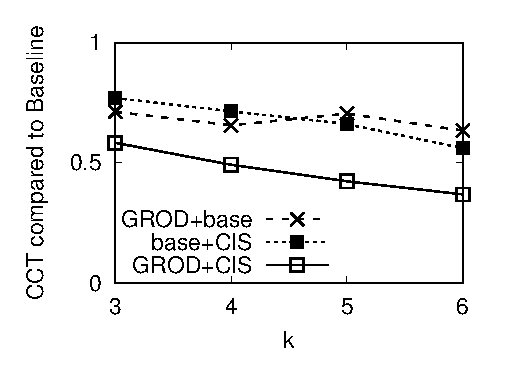
\includegraphics[width=1\textwidth]{28_k_cct.eps}
\caption{CCT compared to Baselinevs. feasible path number $k$ with 2-8 distribution}\label{fig:28_k_cct}
\end{minipage}
\hspace{1mm}
\begin{minipage}[c]{0.23\textwidth}
\centering

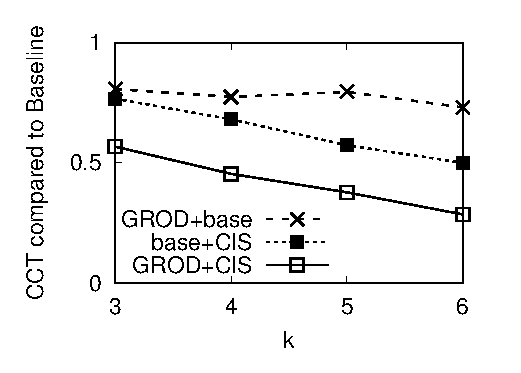
\includegraphics[width=1\textwidth]{normal_k_cct.eps}
\caption{CCT compared to Baseline vs. feasible path number $k$ with normal distribution}\label{fig:normal_k_cct}
\end{minipage}
\hspace{1mm}
\begin{minipage}[c]{0.23\textwidth}
\centering

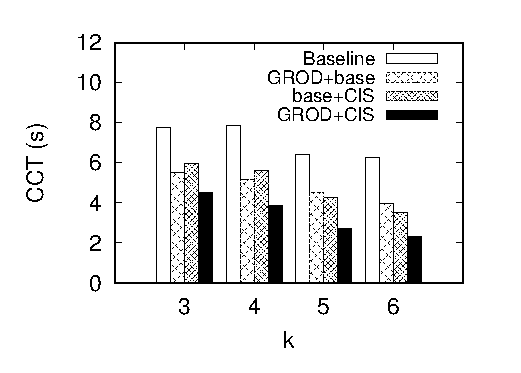
\includegraphics[width=1\textwidth]{28_k_cct_histogram.eps}
\caption{CCT vs. feasible path number $k$ with 2-8 distribution$\qquad\qquad$}\label{fig:28_k_cct_histogram}
\end{minipage}
\hspace{1mm}
\begin{minipage}[c]{0.23\textwidth}
\centering

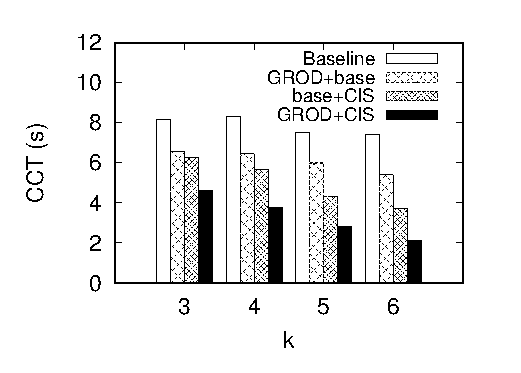
\includegraphics[width=1\textwidth]{normal_k_cct_histogram.eps}
\caption{CCT vs. feasible path number $k$ with normal distribution}\label{fig:normal_k_cct_histogram}
\end{minipage}
\vspace{0cm}
\begin{minipage}[c]{0.23\textwidth}
\centering

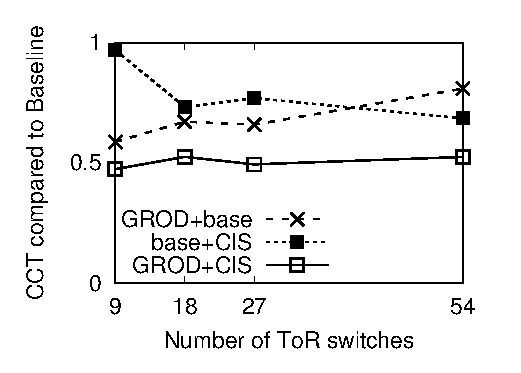
\includegraphics[width=1\textwidth]{28_count_cct.eps}
\caption{CCT compared to Baseline vs. Number of ToR switches with 2-8 distribution}\label{fig:28_count_cct}
\end{minipage}
\hspace{1mm}
\begin{minipage}[c]{0.23\textwidth}
\centering

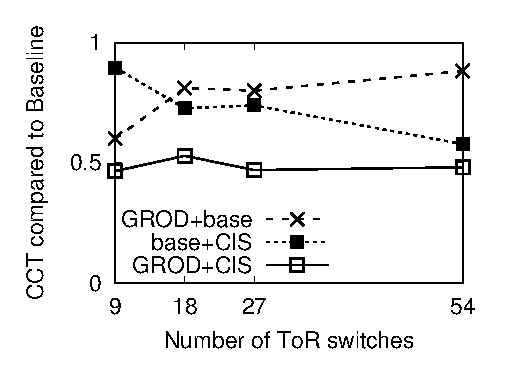
\includegraphics[width=1\textwidth]{normal_count_cct.eps}
\caption{CCT compared to Baseline vs. Number of ToR switches with normal distribution}\label{fig:normal_count_cct}
\end{minipage}
\hspace{1mm}
\begin{minipage}[c]{0.23\textwidth}
\centering

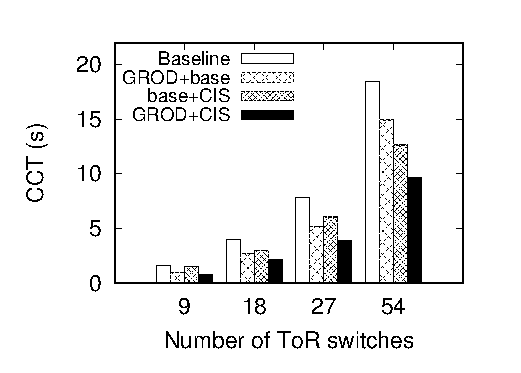
\includegraphics[width=1\textwidth]{28_count_cct_histogram.eps}
\caption{CCT vs. Number of ToR switches with 2-8 distribution$\qquad\qquad$}\label{fig:28_count_cct_histogram}
\end{minipage}
\hspace{1mm}
\begin{minipage}[c]{0.23\textwidth}
\centering
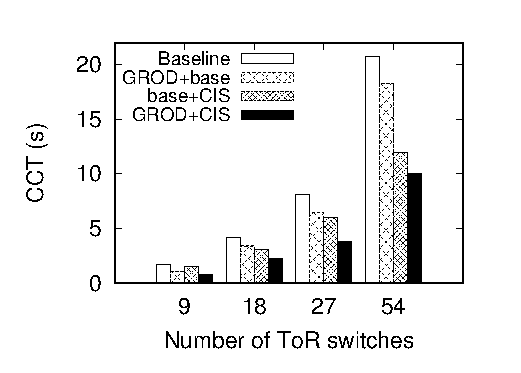
\includegraphics[width=1\textwidth]{normal_count_cct_histogram.eps}
\caption{CCT vs. Number of ToR switches with normal distribution}\label{fig:normal_count_cct_histogram}
\end{minipage}
\vspace{-0.5cm}
\end{figure*}
\begin{figure*}
\centering
\begin{minipage}[c]{0.23\textwidth}
\centering

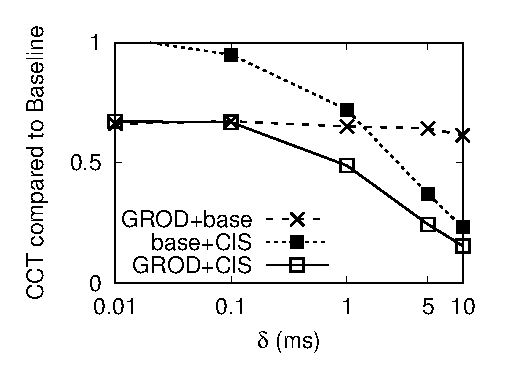
\includegraphics[width=1\textwidth]{28_delta_cct.eps}
\caption{CCT compared to Baseline vs. configuration delay $\delta$ with 2-8 distribution}\label{fig:28_delta_cct}
\end{minipage}
\hspace{1mm}
\begin{minipage}[c]{0.23\textwidth}
\centering

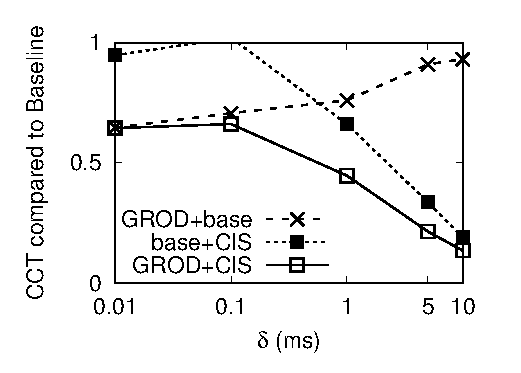
\includegraphics[width=1\textwidth]{normal_delta_cct.eps}
\caption{CCT compared to Baseline vs. configuration delay $\delta$ with normal distribution}\label{fig:normal_delta_cct}
\end{minipage}
\hspace{1mm}
\begin{minipage}[c]{0.23\textwidth}
\centering

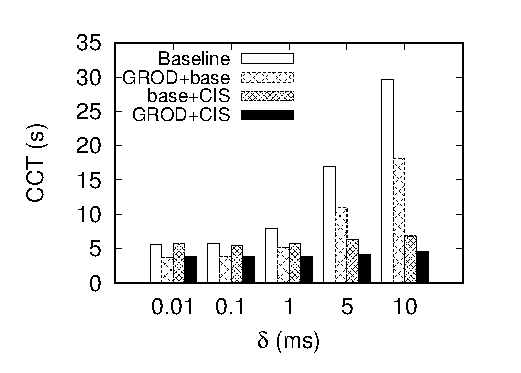
\includegraphics[width=1\textwidth]{28_delta_cct_histogram.eps}
\caption{CCT vs. configuration delay $\delta$ with 2-8 distribution $\qquad\qquad$}\label{fig:28_delta_cct_histogram}
\end{minipage}
\hspace{1mm}
\begin{minipage}[c]{0.23\textwidth}
\centering

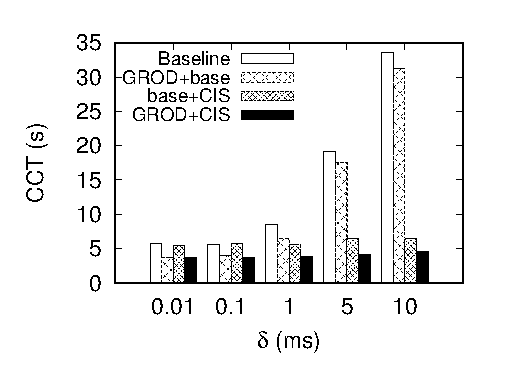
\includegraphics[width=1\textwidth]{normal_delta_cct_histogram.eps}
\caption{CCT vs. configuration delay $\delta$ with normal distribution$\qquad$ $\qquad$}\label{fig:normal_delta_cct_histogram}
\end{minipage}
\vspace{0cm}

\begin{minipage}[c]{0.23\textwidth}
\centering

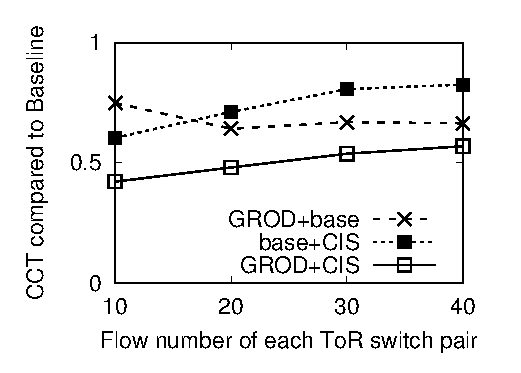
\includegraphics[width=1\textwidth]{28_flow_cct.eps}
\caption{CCT compared to Baseline vs. flow number per ToR pair with 2-8 distribution}\label{fig:28_flow_cct}
\end{minipage}
\hspace{1mm}
\begin{minipage}[c]{0.23\textwidth}
\centering

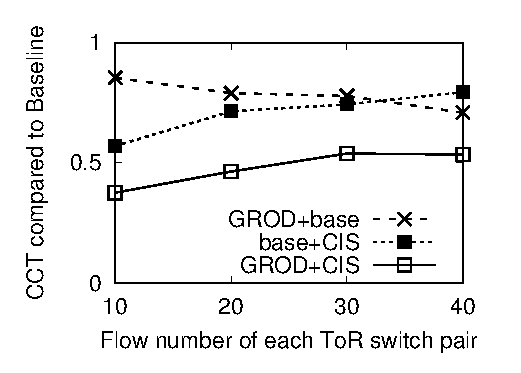
\includegraphics[width=1\textwidth]{normal_flow_cct.eps}
\caption{CCT compared to Baseline vs. flow number per ToR pair with normal distribution}\label{fig:normal_flow_cct}
\end{minipage}
\hspace{1mm}
\begin{minipage}[c]{0.23\textwidth}
\centering

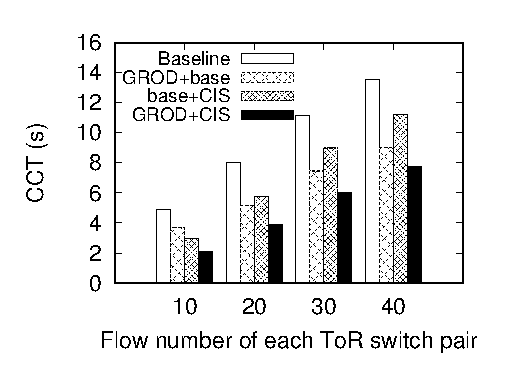
\includegraphics[width=1\textwidth]{28_flow_cct_histogram.eps}
\caption{CCT vs. flow number of each ToR switch pair with 2-8 distribution$\qquad$$\qquad$}\label{fig:28_flow_cct_histogram}
\end{minipage}
\hspace{1mm}
\begin{minipage}[c]{0.23\textwidth}
\centering

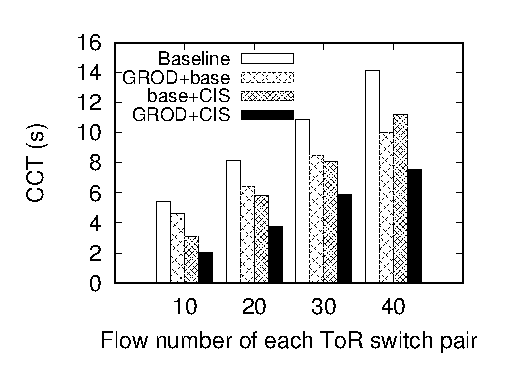
\includegraphics[width=1\textwidth]{normal_flow_cct_histogram.eps}
\caption{CCT vs. flow number of each ToR switch pair with normal distribution$\qquad$$\qquad$}\label{fig:normal_flow_cct_histogram}
\end{minipage}
\vspace{-0.5cm}

\end{figure*}

\subsection{Performance Comparison}
The simulation are performed under four dimensions. Here we illustrate the impacts of four dimensions.

\textbf{Impact of feasible lightpath number $k$:}
To evaluate how the algorithms are influenced by the feasible lightpath number $k$. We fix the other parameters to be defaulted. The result are shown in Figure \ref{fig:28_k_cct}-\ref{fig:normal_k_cct_histogram}, where the horizontal axis is $k$, ranging from 3 to 6. In Fig. \ref{fig:28_k_cct} and \ref{fig:normal_k_cct}, the vertical axis is the coflow completion time (CCT) compared to Baseline. As a result, for all the three algorithms, the CCTs compared to Baseline go down as k increases. For example, in Fig. \ref{fig:normal_k_cct}, the CCT of GROD+CIS compared to Baseline goes down from 0.55 to 0.28. That's because when k goes up, the load on each feasible lightpath is lower and the corresponding duration is smaller. What's more, when $k$ is small, GROD+Base sometimes performs better than Base+CIS. For example, in Fig. \ref{fig:28_k_cct}, when $k=3$, GROD+base will reduce 6\% CCT compared to Base+CIS. However, when $k=6$, GROD+base will increase 6\% CCT compared to base+CIS. That's because our Baseline for CIS is more sensitive to $k$. Our proposed GROD+CIS algorithm can reduce 40-70\% CCT compared to Baseline. Even for base+CIS and GROD+base, our GROD+CIS algorithm can reduce the CCT by 20\%-40\%, especially when $k=6$.

In Fig. \ref{fig:28_k_cct_histogram} and \ref{fig:normal_k_cct_histogram}, the vertical axis is CCT(s). As the feasible lightpath number $k$ increases, there are more lightpaths in the network. As a result, the CCTs of four algorithms decrease. For example, in Fig. \ref{fig:28_k_cct_histogram}, the CCT of baseline goes down from 7.8s to 6.2s when $k$ increases from 3 to 6.

\textbf{Impact of ToR switch number:}
To evaluate how the algorithms are influenced by the ToR switch number. We fix the other parameters to be defaulted. The results are shown in Figure \ref{fig:28_count_cct}-\ref{fig:normal_count_cct_histogram}, where the horizontal axis is the number of ToR switches in the network, ranging from 9 to 54. In Fig. \ref{fig:28_count_cct} and \ref{fig:normal_count_cct}, the vertical axis is the coflow completion time (CCT) compared to Baseline. As a result, the CCT compared to Baseline change little as the number of ToR switches increases for GROD+CIS. But for GROD+base (base+CIS), it goes up (down) as the number of ToR switches increases. What's more, when ToR switch number is small, GROD+base performs better than base+CIS. For example, in Fig. \ref{fig:28_count_cct}, when there are 27 ToR switches, GROD+base will reduce 10\% CCT compared to base+CIS. However, when there are 54 ToR switches, GROD+base will increase 10\% CCT compared to base+CIS. Our proposed GROD+CIS algorithm can reduce 50\% CCT compared to Baseline. Even for base+CIS and GROD+base, our GROD+CIS algorithm can reduce the CCT by 15\%-30\%. That's because our proposed algorithm helps to reduce the CCT by combining coflow scheduling and circuits scheduling.

In Fig. \ref{fig:28_count_cct_histogram} and \ref{fig:normal_count_cct_histogram}, the vertical axis is CCT(s). As the number of ToR switches increases, there are more flows in the network. As a result, the CCTs of four algorithms increase dramatically. For Baseline, the CCT go up from 2s to 18s when ToR switch number increases from 9 to 54.

\textbf{Impact of configuration delay:}
To evaluate how the algorithms are influenced by the configuration delay $\delta$. We fix the other parameters to be defaulted. The result are shown in Figure \ref{fig:28_delta_cct}-\ref{fig:normal_delta_cct_histogram}, where the horizontal axis is $\delta$, ranging from 0.01ms to 10ms. In Fig. \ref{fig:28_delta_cct} and \ref{fig:normal_delta_cct}, the vertical axis is the coflow completion time (CCT) compared to Baseline. As a result, for GROD+CIS and Bseline+CIS, the CCTs compared to Baseline go down as $\delta$ increases. But for GROD+base, it goes up. For example, in Fig. \ref{fig:normal_delta_cct}, the CCT of GROD+CIS compared to Baseline goes down from 0.65 to 0.17. That's because when delta goes up, the reconfiguration times plays an more important role and our proposed CIS algorithm will not change the reconfiguration times, while the baseline of CIS does. For example, in Fig. \ref{fig:normal_delta_cct}, when $\delta=1$, GROD+base and GROD+CIS will reduce approximately 80\% CCT compared to base+CIS and GROD+base.

In Fig. \ref{fig:28_delta_cct_histogram} and \ref{fig:normal_delta_cct_histogram}, the vertical axis is CCT(s). As $\delta$ increases, GROD+base and Baseline dramatically increase the CCT, while base+CIS and GROD+CIS keep stable and much smaller CCT. It shows that our CIS can reduce the reconfiguration times.


\textbf{Impact of flow number per ToR switch pair:}
To evaluate how the algorithms are influenced by the flow number per ToR switch pair. We fix the other parameters to be defaulted. The results are shown in Figure \ref{fig:28_flow_cct}-\ref{fig:normal_flow_cct_histogram}, where the horizontal axis is the flow number per ToR switch pair, ranging from 10 to 40. In Fig. \ref{fig:28_flow_cct} and \ref{fig:normal_flow_cct}, the vertical axis is the coflow completion time (CCT) compared to Baseline. As a result, for base+CIS and GROD+CIS, the CCTs compared to Baseline go up as the flow number per ToR switch pair increases. However, for GROD+base, it goes down, especially for normal distribution. For example, in Fig. \ref{fig:normal_flow_cct}, the CCT of GROD+CIS compared to Baseline goes up from 0.39 to 0.55. But for GROD+base, it goes down from 0.85 to 0.72. That's because when the flow number per ToR switch pair increases, the $\delta$ will be less significant compared to the flow traffic. Just like Fig. \ref{fig:normal_delta_cct_histogram}, when $\delta$ decreases, the CCT compared to Baseline of GROD+CIS and base+CIS increase a bit, but the that of GROD+base keep stable. So it's not because our CIS algorithm doesn't work but essentially because the $\delta$ is less significant compared to the flow traffic when the flow number increases. What's more, when the flow number per ToR switch pair is small, base+CIS sometimes performs better than GROD+base. For example, in Fig. \ref{fig:28_flow_cct}, when the flow number per ToR switch pair is 10, base+CIS reduces 20\% CCT compared to GROD+base. However, when the flow number per ToR switch pair is 40, base+CIS increases 20\% CCT compared to GROD+base. %That's because our base for CIS is more sensitive to the lightpath number. Our proposed GROD+CIS algorithm can reduce 40-60\% CCT compared to Baseline. Even for Baseline+CIS and GROD+base, our GROD+CIS algorithm can reduce the CCT by 20\%-40\%, especially when $flow=6$.

In Fig. \ref{fig:28_flow_cct_histogram} and \ref{fig:normal_flow_cct_histogram}, the vertical axis is CCT(s). As the flow number per ToR switch pair increases, there are more flows in the network. As a result, the CCTs of four algorithms increases. For Baseline in Fig. \ref{fig:normal_flow_cct_histogram}, the CCT goes up from 5.5s to 14s when  the flow number per ToR switch pair increases from 10 to 40.

\subsection{Running Time}
In this part, we evaluate how the feasible lightpath number $k$ and ToR switch number can influence the running time. The results are shown in Fig. \ref{fig:28_k_time_histogram} and \ref{fig:28_count_time_histogram}, where the vertical axis is running time. In Fig. \ref{fig:28_k_time_histogram}, as $k$ increases, the running time increases too. But compared to the Fig. \ref{fig:28_count_time_histogram}, the running time increases dramatically when the number of ToR switches increases. That's because the lightpath number is $O(n^2)$ for the number of ToR switches while $k$ can only change the number of lightpaths linearly.

\begin{figure}
\centering
\begin{comment}
\begin{minipage}[c]{0.23\textwidth}
\centering
\includegraphics[width=1\textwidth]{28_k_time.eps}
\caption{Running time compared to Baseline vs. feasible lightpath number $k$ with 2-8 distribution}\label{fig:28_k_time}
\end{minipage}
\hspace{1mm}
\end{comment}
\begin{minipage}[c]{0.23\textwidth}
\centering

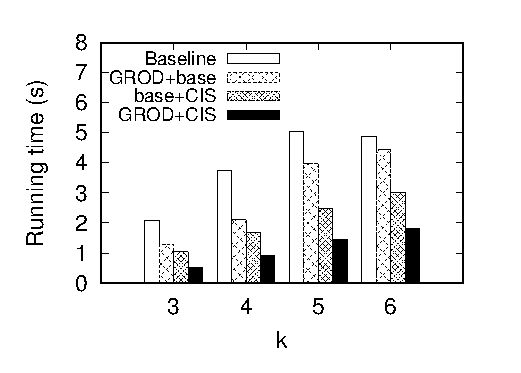
\includegraphics[width=1\textwidth]{28_k_time_histogram.eps}
\caption{Running time vs. feasible lightpath number $k$ with 2-8 distribution}\label{fig:28_k_time_histogram}
\end{minipage}
\vspace{-0.3cm}
\begin{comment}
\begin{minipage}[c]{0.23\textwidth}
\centering

\includegraphics[width=1\textwidth]{28_count_time.eps}
\caption{Running time compared to Baseline vs. ToR switch number with 2-8 distribution}\label{fig:28_count_time}
\end{minipage}
\end{comment}
\hspace{1mm}
\begin{minipage}[c]{0.23\textwidth}
\centering

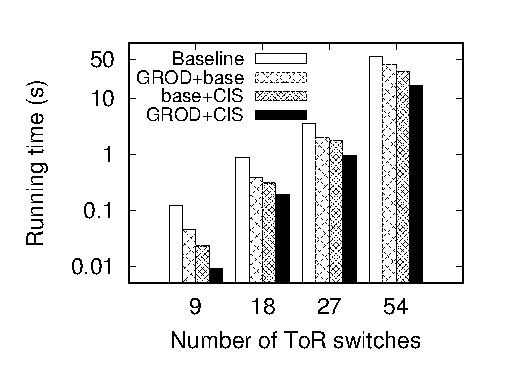
\includegraphics[width=1\textwidth]{28_count_time_histogram.eps}
\caption{Running time vs. ToR switch number with 2-8 distribution}\label{fig:28_count_time_histogram}
\end{minipage}
\vspace{-0.3cm}


\end{figure}

%\subsection{Conclusion}
%Our GROD+CIS algorithm can reduce the CCT by 40-80\% compared to Baseline in four dimensions. The two hybrid algorithms, GROD+base and base+CIS, achieve the CCTs in the middle of Baseline and GROD+CIS, which shows the effectiveness of both of steps. Because of the space is limited, we do not repeat in detail.



\section{Related works}\label{sec:relwork}
A coflow is a flow set transferring data between two stages \cite{chowdhury2012coflow}. For a better application performance, we need to reduce the coflow completion time (CCT). Many works have been done in the classical networks. However, in optical circuit switched networks, how to reduce the CCT remains an open problem. There are two important ways to reduce the CCT. One is coflow scheduling, the other is scheduling the circuits in the OCS network. In the part, we will introduce the corresponding works respectively.

Many works have studied the coflow scheduling in the data center networks. The author of \cite{chowdhury2012coflow} summarized the traffic patterns and explicitly proposed the concept of coflow. After that, researches like \cite{chowdhury2014efficient} and \cite{dogar2014decentralized} started to apply the coflow concept in their optimizations. All of the above works focused on when to forward the flows while neglecting the routing part. Only the author of \cite{zhao2015rapier} added the routing problem for coflows in the DCNs. However, the classical networks are packet switched networks. The OCS networks are circuits switched networks \cite{huang2016sunflow}. The coflow scheduling for packet switched networks are not suitable for circuits switched networks because optical switches have port constraints and the lightpath is not always available. To the best of our knowledge, no research has studied the coflow scheduling (including routing part) in the OCS network ever before. Most of the researches about optimizing the CCT in the OCS network focus on the circuits scheduling.

Another important method is circuits scheduling. Because the optical circuit switches have port constraint, a natural topic is scheduling the circuits to minimize the CCT of the coflow. The researches like \cite{farrington2012hunting} and \cite{porter2013integrating} scheduled the circuits with the classic BvN matrix decomposition algorithm \cite{birkhoff1946tres}. To use BvN, they would pre-process the demand matrixto meet the inpt assumption of BvN and decompose the pre-processed matrix into assignments and weights for each assignment. The author of \cite{liu2015scheduling} added dummy demand to the demand matrix in it's pre-process step. The above researches are based on the \emph{all-stop} model, which assumes communication stops on all optical circuits during reconfiguration. It's unnecessary because circuits unchanged are not impacted and keep serving traffic \cite{huang2016sunflow}. Besides, the above researches all focused on the scheduling in a single switch not the whole optical network. The author of \cite{wang2015end} focused on the scheduling for optical networks based on the \emph{all-stop} model. Sunflow \cite{huang2016sunflow} studied the circuits scheduling based on the \emph{not-all-stop} model, but it's scheduling is a single optical circuit switch scheduling not the circuits scheduling of a OCS network. To the best of our knowledge, no research has studied the circuits scheduling of the whole OCS network.

Coflow scheduling and circuits scheduling both influence the CCT. The coordination of coflow scheduling and circuits scheduling is complicated but necessary.  Our paper will integrate these two ways to minimize the CCT.






\section{Conclusion}\label{sec:conclusion}
In this paper, we formulate the coflow and circuits scheduling (COCIS)problem and prove it's NP-hardness. What's more, we prove it's two subproblems, coflow scheduling (COS) and circuits scheduling (CIS), are NP-hard too. To solve these two subproblems, we propose the corresponding approximation algorithms with analyzed approximation ratio. Later in our simulation, we show that our proposed GROD+CIS algorithm can reduce the CCT by 40\%-80\%.


\bibliographystyle{IEEEtran}
\bibliography{refs}

%\section{Appendix}
%
\begin{IEEEproof}
For the CRS problem, the OCS network scheduling scheme is fixed. We consider a special case that the coflow only has the flow set $f_{i,j}=\{f_{i,j}^1,f_{i,j}^2,...\}$ from source ToR switch $i$ to destination ToR switch $j$. There is a lightpath set $P_{i,j}$ which includes multiple lightpaths $p\in P_{i,j}$ connecting ToR switch $i$ and ToR switch $j$. Each lightpath has active periods. What's more, there is an interval T between two active periods. Let's consider a special case that interval T of each lightpath is 0 and each lightpath starts at the initial moment. Thus, each light path is active all the time, our objective is to minimize the completion time. Then our problem because the \emph{multi machine scheduling} problem, which is known to be NP-hard \cite{mosheiov1998multi}. The special case of our problem is NP-hard, so our problem is NP-hard too.
\end{IEEEproof}

\begin{IEEEproof}
For the CS problem, Similar to the proof of \ref{CRS:nphard}. We consider a special case that the OCS network scheduling scheme is fixed and the coflow only has the flow set $f_{i,j}=\{f_{i,j}^1,f_{i,j}^2,...\}$ from source ToR switch $i$ to destination ToR switch $j$. There is a lightpath set $P_{i,j}$ which includes multiple lightpaths $p\in P_{i,j}$ connecting ToR switch $i$ and ToR switch $j$. Each lightpath has active periods. We consider an special case that the active periods of each lightpath is infinite and each lightpath starts at the initial moment. Thus the flows won't be interrupted (active period is long enough) and the first active period of each lightpath is enough for the flows scheduling. Under this special case, our problem becomes the \emph{multi machine scheduling} problem, which is known to be NP-hard \cite{mosheiov1998multi}. The special case of our problem is NP-hard, so we have proven the NP-hardness of our problem.
\end{IEEEproof}


\appendices
%
\section{Proof of Lemma \ref{COS:nphard}}\label{proof:COS}
\begin{IEEEproof}
For the COS problem, the OCS network scheduling scheme is fixed. We consider a special case that the coflow only has the flow set $f_{i,j}=\{f_{i,j}^1,f_{i,j}^2,...\}$ from source ToR switch $i$ to destination ToR switch $j$. There is a lightpath set $P_{i,j}$ which includes multiple lightpaths $p\in P_{i,j}$ connecting ToR switch $i$ and ToR switch $j$. Each lightpath has active periods. What's more, there is an interval T between two active periods. Let's consider a special case that interval T of each lightpath is 0 and each lightpath starts at the initial moment. Thus, each light path is active all the time, our objective is to minimize the completion time. Then our problem because the \emph{multi machine scheduling} problem, which is known to be NP-hard \cite{mosheiov1998multi}. The special case of our problem is NP-hard, so our problem is NP-hard too.
\end{IEEEproof}


%
\section{Proof of Lemma \ref{CIS:nphard}}\label{proof:CIS}
\begin{IEEEproof}
For the CIS problem, the route and required duration of each lightpath are given. We need to schedule the optical circuit switches of the whole network. Let's consider a special case that the OCS network has only one optical switch. Then the route of each lightpath will become the input-output pair. When the reconfiguration delay $\delta=\infty$, the preemption penalty $=\infty$. Thus the CIS problem reduces to the non-preemptive open-shop problem to minimize work span \cite{gonzalez1976open}, where each job (input port $i$) requires processing time (duration of the lightpath) on a specific machine (output port $j$). The open-shop problem is non-preemptive, which means a machine (output port $j$) would always finish processing a job (lightpath from one input port $i$) before moving to another job. The problem is NP-hard \cite{gonzalez1976open}. The special case of the CIS problem is NP-hard, so CIS is NP-hard too.
\end{IEEEproof}



\end{document}
